\chapter{Empirical study}
\label{cp:dataset and experiment}
\section{Dataset}
In order to verify the feasibility of the proposed approach, authentic mobile phone cover images are acquired on a colour CMOS (Complementary metal–oxide–semiconductor) camera. Each coloured RGB image has $100 \times 100$ pixels in size, three-colour bands per pixel, and eight bits of intensity per colour band. The database consists of 235 mobile-phone cover images, of which 195 have no defects and 40 have various defects. All programming is done in Matlab.

A mobile-phone cover image shown in Figure~\ref{fig:handy-cover} is used for experiment. Firstly, the background, camera hole, and logo are subtracted, and then the original image is resized to several $100 \times 100$ pixels sample images, which are called standard images, shown in Figure~\ref{fig:sample}. The defect image samples are acquired with the same procedure as standard image samples, shown in Figure~\ref{fig:sample}.



\begin{figure}[h]
\centering
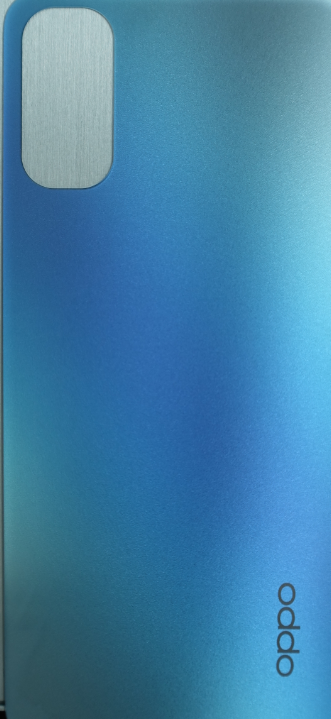
\includegraphics[width=0.2\textwidth]{images/original1.png}
\caption{Mobile-phone cover image}
\label{fig:handy-cover}
\end{figure}

\section{Experiment}
\subsection{Determine the size of the moving window}
An experiment is conducted to find out the suitable size of the sliding window. Three different windows with size $5 \times 5$ pixels, $10 \times 10$ pixels, and $20 \times 20$ pixels are applied on several defect images (see Figure~\ref{fig:sample}). After the specific size of window go through the image, the maximum variance among all the windows is considered as the desired statistic of this image by this specific size of the window. The window's size with the largest variance on the same image will be the most suitable size of the sliding window for detecting defect in this image. 

The result is shown in Table~\ref{fig:Tab1}. From that we can note that the largest maximum variance of samples with surface dent and surface swelling appear at $10 \times 10$ windows. Although the maximum value of sample with surface scratch appears in the $5 \times 5$ window, consider its value is close to the second largest value, and the value itself is relatively small, we still believe $10 \times 10$ is the most appropriate size for the sliding window.

\begin{table}[htp]
\centering
\setlength{\tabcolsep}{0pt}
\begin{tabular*}{\textwidth}{
  @{\extracolsep{\fill}}
  l
  S[table-format=1.3e-2]
  S[table-format=6.0]
  S[table-format=1.4e-1]
  S[table-format=1.1]
  S[table-format=1.4e-1]
  @{}
}
\toprule
Sample  &
{$5\times5$ pixels} &
{$10\times10$ pixels} &
{$20\times20$ pixels}  \\
\midrule
surface dent & 220.96 & 494.57 & 191.27  \\
surface scratch & 71.12 & 48.75 & 45.47  \\
surface swelling & 1.17e+03 & 1.33e+03 & 9.20e+02  \\
\bottomrule
\end{tabular*}
\caption{The maximum variance of three size windows of different defect samples (see Figure~\ref{fig:sample}). As we can observe, the size of the sliding window is depend on the size of the defect area, thus we choose three sizes of window to compare their performance on different defects.}
\label{fig:Tab1}
\end{table}


\begin{figure}[h]
\centering
\subfigure{
\begin{minipage}[b]{0.2\textwidth}
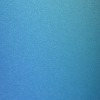
\includegraphics[width=1\textwidth]{images/image_part_022.jpg} \\
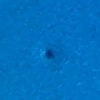
\includegraphics[width=1\textwidth]{images/b1.jpg}
\end{minipage}
}
\subfigure{
\begin{minipage}[b]{0.2\textwidth}

\includegraphics[width=1\textwidth]{images/g11.png} \\
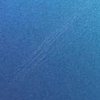
\includegraphics[width=1\textwidth]{images/b16.jpg}
\end{minipage}
}
\subfigure{
\begin{minipage}[b]{0.2\textwidth}
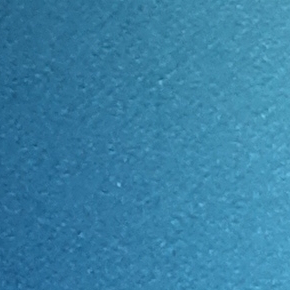
\includegraphics[width=1\textwidth]{images/image_part_084.jpg} \\
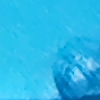
\includegraphics[width=1\textwidth]{images/b3.jpg}
\end{minipage}
}
\caption{Illustration of standard sample images and defect images. The first row is the standard images, and the second row is images with different defects: From left to right are surface dent, surface scratch and surface swelling.}
\label{fig:sample}
\end{figure}

\begin{comment}
\begin{figure}[htbp]
\centering
\subfigure{
\begin{minipage}[t]{0.2\linewidth}
\centering
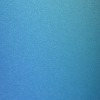
\includegraphics[width=1in]{images/image_part_022.jpg}
%\caption{fig1}
\end{minipage}%
}%
\subfigure{
\begin{minipage}[t]{0.2\linewidth}
\centering

\includegraphics[width=1in]{images/g11.png}
%\caption{fig2}
\end{minipage}%
}%
\subfigure{
\begin{minipage}[t]{0.2\linewidth}
\centering
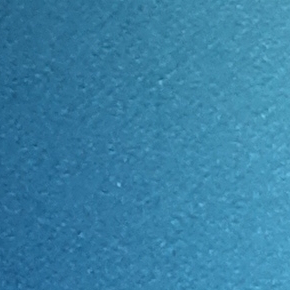
\includegraphics[width=1in]{images/image_part_084.jpg}
%\caption{fig2}
\end{minipage}
}%
\centering
\caption{Standard images}
\label{fig:sample}
\end{figure}

\begin{figure}[htbp]
\centering
\subfigure[a]{
\begin{minipage}[t]{0.2\linewidth}
\centering
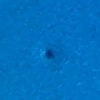
\includegraphics[width=1in]{images/b1.jpg}
%\caption{fig1}
\end{minipage}%
}%
\subfigure[b]{
\begin{minipage}[t]{0.2\linewidth}
\centering
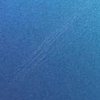
\includegraphics[width=1in]{images/b16.jpg}
%\caption{fig2}
\end{minipage}%
}%
\subfigure[c]{
\begin{minipage}[t]{0.2\linewidth}
\centering
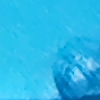
\includegraphics[width=1in]{images/b3.jpg}
%\caption{fig2}
\end{minipage}
}%
\centering
\caption{Defect images: (a)Surface dent. (b)Surface scratch. (c)Surface swelling. }
\label{fig:defect_images}
\end{figure}
\end{comment}




\subsection{Sensitivity test of detail coefficient matrices to defects}
\label{subsec:hvd_experiment}
This section conducts an experiment to test and compare the sensitivity of three detail coefficient matrices $\mathbf H$, $\mathbf V$, and $\mathbf D$ to various defects. The experiment will be performed in the following way: several test images with various defects shown in Figure~\ref{fig:sample} are decomposed by HWT (section~\ref{sec:dwt}) to the final level. The decomposed detail matrix $\mathbf H$, $\mathbf V$, and $\mathbf D$ are compared to find out which matrix among the horizontal, vertical and diagonal matrices can best reflect defects in the corresponding image.


% for hand-mand 4 images
\begin{comment}

\begin{figure}[h]
\centering
\subfigure[a]{
\begin{minipage}[t]{0.2\linewidth}
\centering
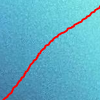
\includegraphics[width=1in]{images/e1 (1).PNG}
%\caption{fig1}
\end{minipage}%
}%
\subfigure[b]{
\begin{minipage}[t]{0.2\linewidth}
\centering
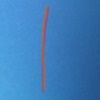
\includegraphics[width=1in]{images/e1 (2).png}
%\caption{fig2}
\end{minipage}%
}%
\subfigure[c]{
\begin{minipage}[t]{0.2\linewidth}
\centering
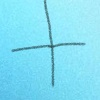
\includegraphics[width=1in]{images/e1 (3).png}
%\caption{fig2}
\end{minipage}
}%
\subfigure[c]{
\begin{minipage}[t]{0.2\linewidth}
\centering
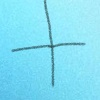
\includegraphics[width=1in]{images/e1 (3).png}
%\caption{fig2}
\end{minipage}
}%
\centering
\caption{Hand-mand images}
\label{fig:hand_made}
\end{figure}


\begin{figure}[h]
\centering
\subfigure{
\begin{minipage}[b]{0.2\textwidth}
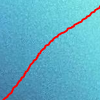
\includegraphics[width=1\textwidth]{images/e1 (1).PNG} \\
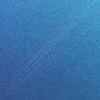
\includegraphics[width=1\textwidth]{images/e4.png}
\end{minipage}
}
\subfigure{
\begin{minipage}[b]{0.2\textwidth}
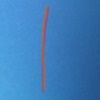
\includegraphics[width=1\textwidth]{images/e1 (2).png} \\
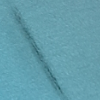
\includegraphics[width=1\textwidth]{images/e5.png}
\end{minipage}
}
\subfigure{
\begin{minipage}[b]{0.2\textwidth}
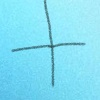
\includegraphics[width=1\textwidth]{images/e1 (3).png} \\
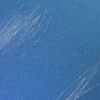
\includegraphics[width=1\textwidth]{images/e6.png}
\end{minipage}
}

\caption{Illustration of test images with different directional scratches. The first row is the hand-made scratch images; the second row is real scratch images from the production line. The serial numbers of the image from top left to bottom right are (a)-(f).}
\label{fig:experiment}
\end{figure}
\end{comment}

Since the decomposed detail matrices at the final level have a few coefficients and our concern is to find out the most sensitive matrix to defect, we calculate the maximum coefficient of $\mathbf H$, $\mathbf V$, and $\mathbf D$ by using Equation (\ref{equ:absD}) and (\ref{equ:maxD}) and 
compare the maximum coefficient {\normalsize H\_max}, V\_max, and D\_max of the same defect image. The matrix containing the maximum coefficient is considered the most suitable candidate among detail matrices. 

\begin{table}[htp]
\centering
\setlength{\tabcolsep}{0pt}
\begin{tabular*}{\textwidth}{
  @{\extracolsep{\fill}}
  l
  S[table-format=1.3e-2]
  S[table-format=6.0]
  S[table-format=1.4e-1]
  S[table-format=1.1]
  S[table-format=1.4e-1]
  @{}
}
\toprule
Sample  &
{H\_max} &
{V\_max} &
{D\_max}  \\
\midrule
surface dent & 134.50 & 226.69 & 151.62  \\
surface scratch & 173.59 & 102.38 & 68.19  \\
surface swelling & 579.09 & 501.88 & 171.19  \\
\bottomrule
\end{tabular*}
\caption{The maximum coefficient among three detail matrices of different defect samples (see Figure~\ref{fig:sample}). }
\label{tab:max_hdv}
\end{table}

Before the experiment is conducted, we assume that the diagonal matrix is sensitive to the diagonal pixel value variation and the difference of horizontal and vertical direction since the diagonal matrix is the result of two repeated differences of pixel value (first by horizontal, then vertical) according to Equation \eqref{equ:haar_wavelet1}-\eqref{equ:haar_wavelet2}.
While in Table~\ref{tab:max_hdv} we can find out that the maximum coefficient of images with diagonal scratch (e.g.surface scratch) does not appear in the $\mathbf D$ matrix, which fails our assumption at the first place. Thus the following conclusion is made: Instead of using one specific detail matrix of HWT to retrieve the image characteristics, we determine to use all three matrices to characterize the sample images.


\subsection{Performance comparison of different methods}
\label{sec:5.3}
In this section three aspects of method I (maximum variance based $\bar{X}$ control chart) and method II (wavelet based Hotelling $T^{2}$ control chart)  will be compared, namely average run length ($ARL$), false detection rate ($FDR$) and average alarm strength ($ARL$). Here we use average run length ($ARL$)

\begin{equation}
    ARL = \frac{1}{P}\,,
    \label{equ:arl}
\end{equation}

where $P$ denoting the probability of an observation plotting outside the control limits to characterize the false alarm in Phase I. The $ARL$ tells us, for a given situation, how long on the average we will plot successive control charts points before we detect a point beyond the control limits~\cite{heckert2002handbook}.

False detection rate can be mathematically represent as
\begin{equation}
    FDR = \frac{n_{f}}{n}\,,
    \label{equ:far}
\end{equation}

in which $n_{f}$ is the number of false detection in Phase II while $n$ is the total sample number in Phase II, $FAR$ is a percentage value describing the percentage of error results in the total sample. And the average alarm strength ($ASS$) is

\begin{equation}
ASS =\frac{\sum_{i=1}^{n} \frac{S_{i}}{UCL}}{n}\,,
\label{equ:aas}
\end{equation}

where $S_{i}$ is $i_{th}$ sample's statistic, whose value is larger than $UCL$, to quantify the corresponding aspect of different methods. $ASS$ is the average ratio of statistic to $UCL$, which is used to measure how sensitive the methods are to defects.


Jensen et al. (2006)~\nocite{jensen2006effects} point out that even larger sample sizes are required to ensure that the Phase II average run length  performance will actually be close to the anticipated values, thus in Phase I, we first use 100 samples in Phase I to retrieve the in-control parameters and the $UCL$ of control chart, then apply the in-control parameters in Phase II (120 samples). The result is shown in Table~\ref{tab:calibration_result}. It turns out that the $ARL$ in Phase I and $FDR$ in Phase II are not satisfactory. Thus a calibration step of is needed.

\begin{table}[htp]
\centering
\setlength{\tabcolsep}{0pt}
\begin{tabular*}{\textwidth}{
  @{\extracolsep{\fill}}
  l
  S[table-format=1.3e-2]
  S[table-format=6.0]
  S[table-format=1.4e-1]
  S[table-format=1.1]
  S[table-format=1.4e-1]
  @{}
}
\toprule
method  &
Phase I false alarm number &
Phase I $ARL$ &
Phase II $FDR$ \\
\midrule
method I & 31 & 3.22 & 9.1\%  \\
method II & 8 & 12.50 & 8.3\%  \\
\bottomrule
\end{tabular*}
\caption{The performance of control charts before calibration. }
\label{tab:calibration_result}
\end{table}

 By calibration on the one hand we replace the false alarm samples in Phase I with standard samples in Phase II, on the other hand we collect another 50 standard samples in Phase I to increase the sample size to improve the performance of both methods. Thus we use 150 standard sample images to retrieve the in-control state of the process by using maximum variance combining the $\bar{X}$ control chart and Haar wavelet decomposition combining Hotelling $T^{2}$ control chart, separately. 

According to Equation \eqref{equ:m_mean}-\eqref{equ:LCL_real}, the mean value ($\overline{m}$) of maximum variance of method I in Phase I is 15.538, the standard deviation ($\sigma_{s}$) is 0.5879, thus the UCL and LCL is 17.302 and 13.775 respectively. By method II in Phase I the sample mean vector of Haar wavelet decomposition characteristic is
\begin{equation}
\centering
\overline{\mathbf{x}} = 
\begin{bmatrix}
50.897 & 97.984 & 19.974
\end{bmatrix}, 
\end{equation}


and the sample covariance matrix is
\begin{equation}
\centering
\mathbf{S} = 
\begin{bmatrix}

448.7801 &	986.332 &	-16.474\\
986.332 &	5251.402 &	-139.947\\
-16.4746 &	-139.947 &	42.3404
\end{bmatrix},
\end{equation}

by using Equation (\ref{equ:UCL_T2}), we can calculate the UCL of method II is 8.157. The control chart of Phase I of method I and method II is shown in Figure~\ref{fig:phasI_methodI} and Figure~\ref{fig:phasI_methodII}. The $ARL$ of method I and method II according to Equation (\ref{equ:arl}) is 3.125 and 30, respectively. 

\begin{figure}
    \centering
    \begin{subfigure}{\textwidth}
         \centering
         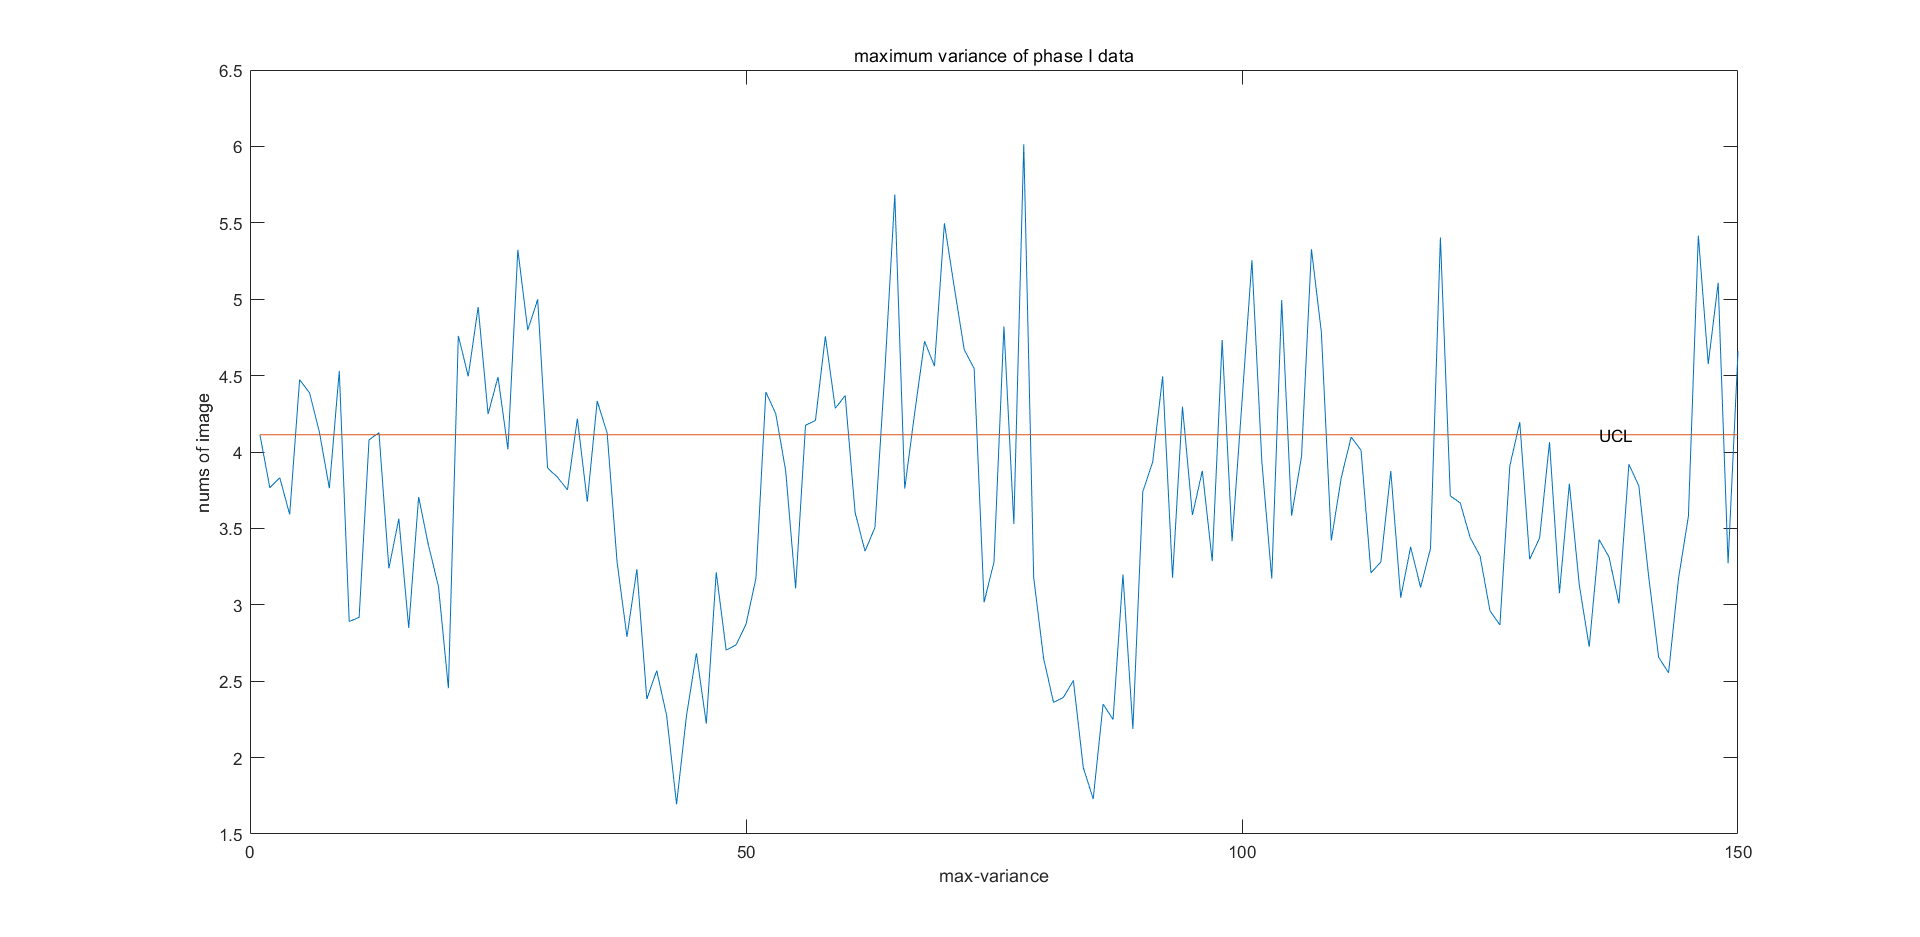
\includegraphics[width=\textwidth]{images/phaseI_max.png}
         \caption{The Phase I maximum variance based $\bar{X}$ control chart, where all the samples are qualified and there are 48 false alarms in the control chart. The orange line is the UCL of $\bar{X}$ control chart}
        \label{fig:phasI_methodI}
    \end{subfigure}
     
    \begin{subfigure}{\textwidth}
         \centering
         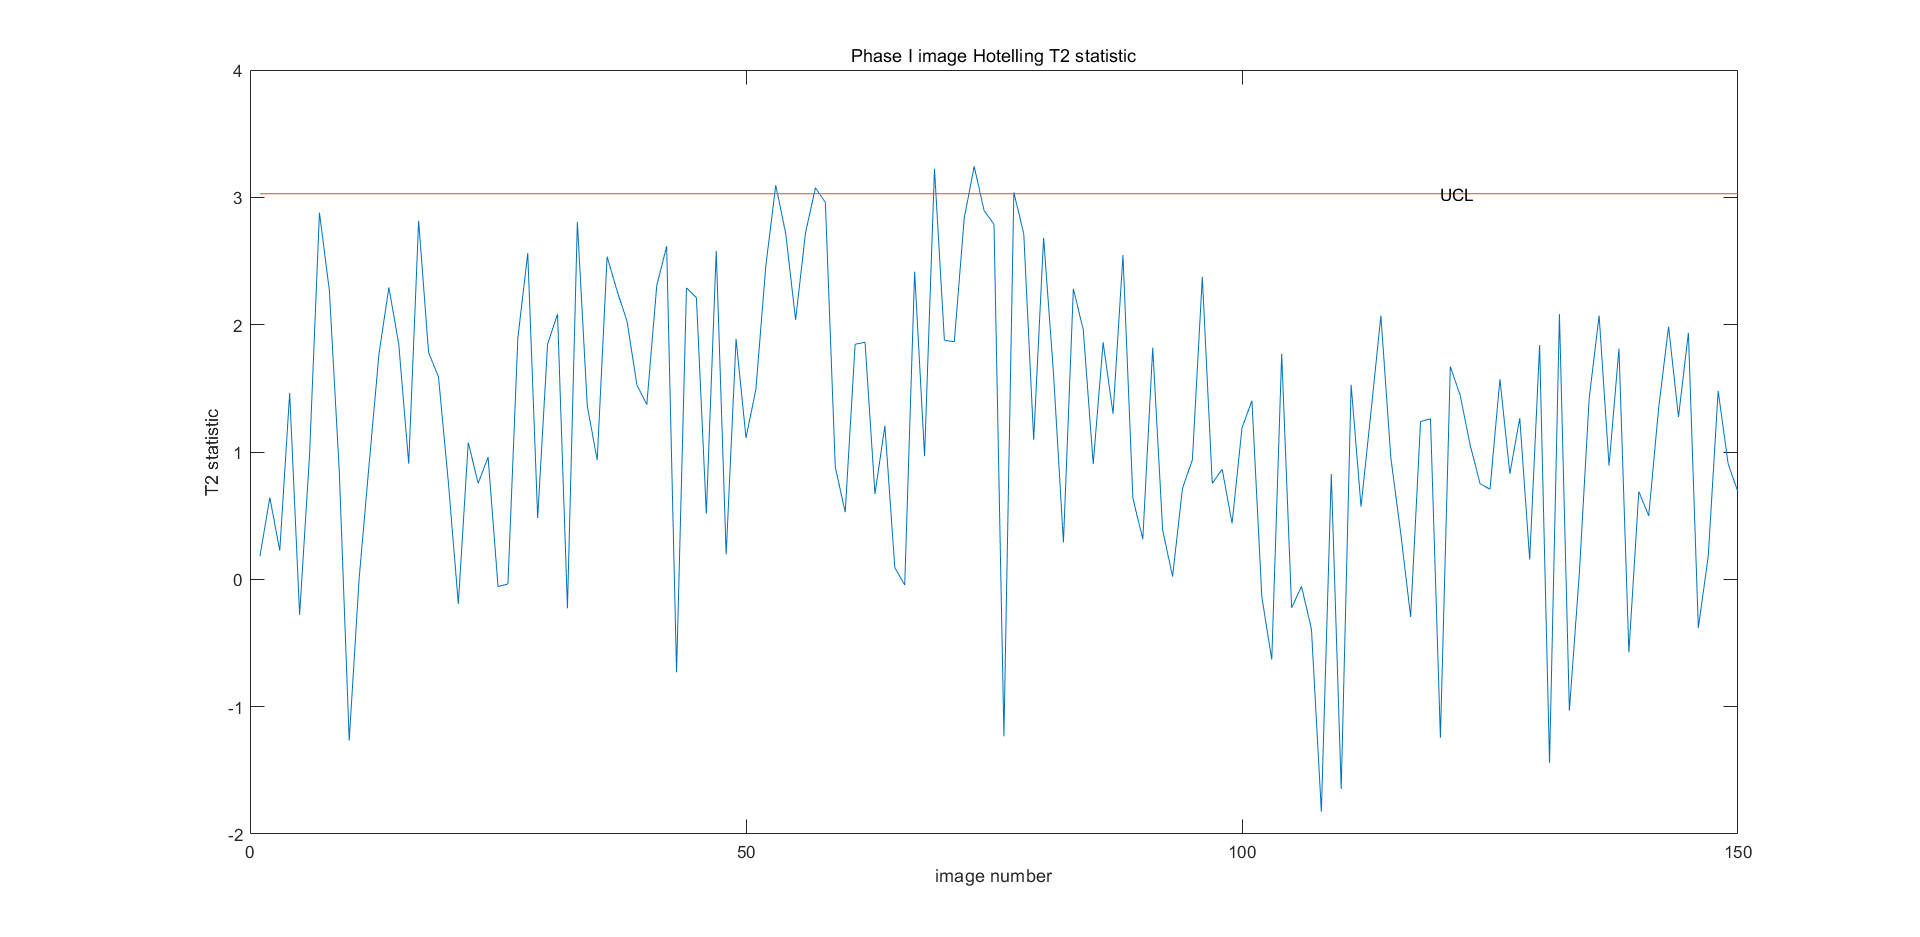
\includegraphics[width=\textwidth]{images/phaseI_t2.png}
         \caption{The Phase I wavelet decomposition based Hotelling $T^{2}$ control chart, where all the samples are qualified and there are 5 false alarms in the control chart. The orange line is the UCL of Hotelling $T^{2}$ control chart}
        \label{fig:phasI_methodII}
    \end{subfigure}
\end{figure}

In Phase II, 85 samples are arranged in a way that the first 40 images are negative, while the rest (45 images) are positive. The control charts of method I and method II are shown in Figure~\ref{fig:max_result_15errors} and \ref{fig:T_result_d1} respectively. According to Equation (\ref{equ:far}) and (\ref{equ:aas}) the false detection rate of method I and method II is almost the same, their value is 5.83\% and 1.18\%, and the $ASS$ of method I and method II is 27.47 and 67.12, respectively. The higher the $ASS$ value, the larger the out-of-state amplitude of this method. The average out-of-state amplitude of method II is almost twice as that of method I, thus we can come to a conclusion that although there is almost no difference between method I and method II in terms of false detection rate in Phase II, method II is more sensitive than method I in defects detection. 
\begin{figure}
    \centering
    \begin{subfigure}{\textwidth}
         \centering
         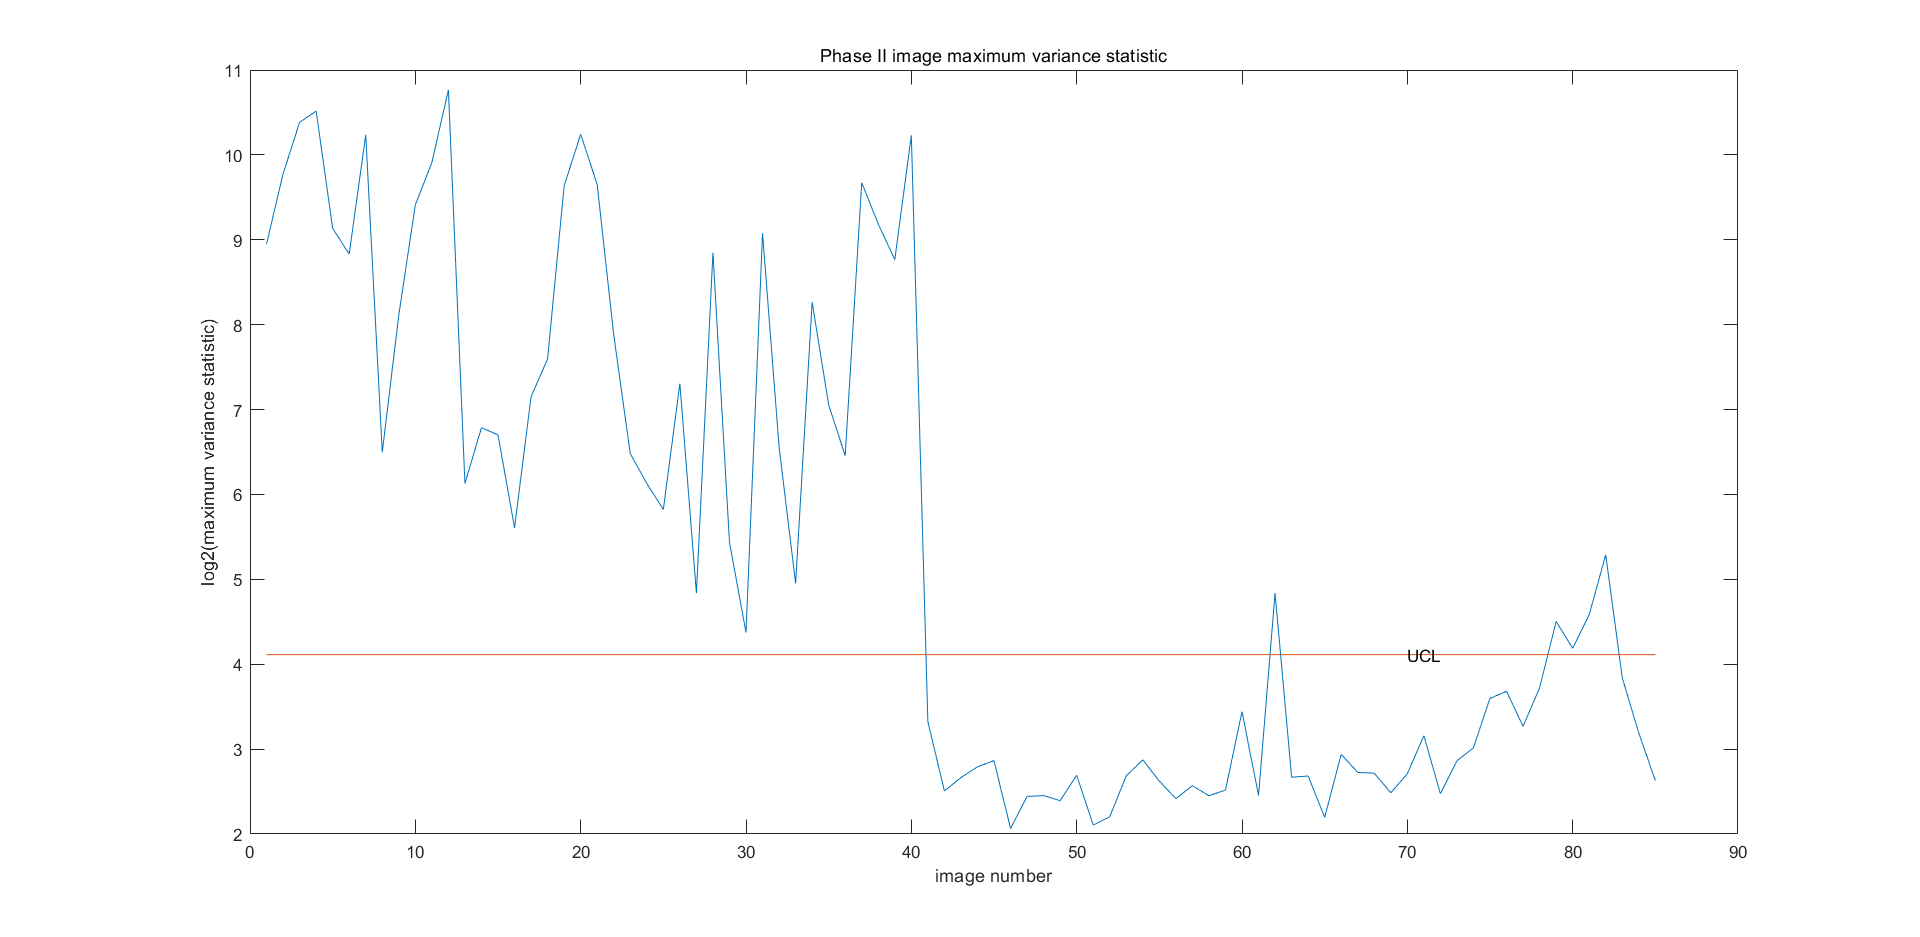
\includegraphics[width=\textwidth]{images/phaseII_max.png}
         \caption{The Phase II maximum variance based $\bar{X}$ control chart, where the first 40 images are sample with defects, other 45 are qualified samples. The orange line indicate the UCL and there are 5 false detection samples in the control chart.}
        \label{fig:max_result_15errors}
    \end{subfigure}
     
    \begin{subfigure}{\textwidth}
         \centering
         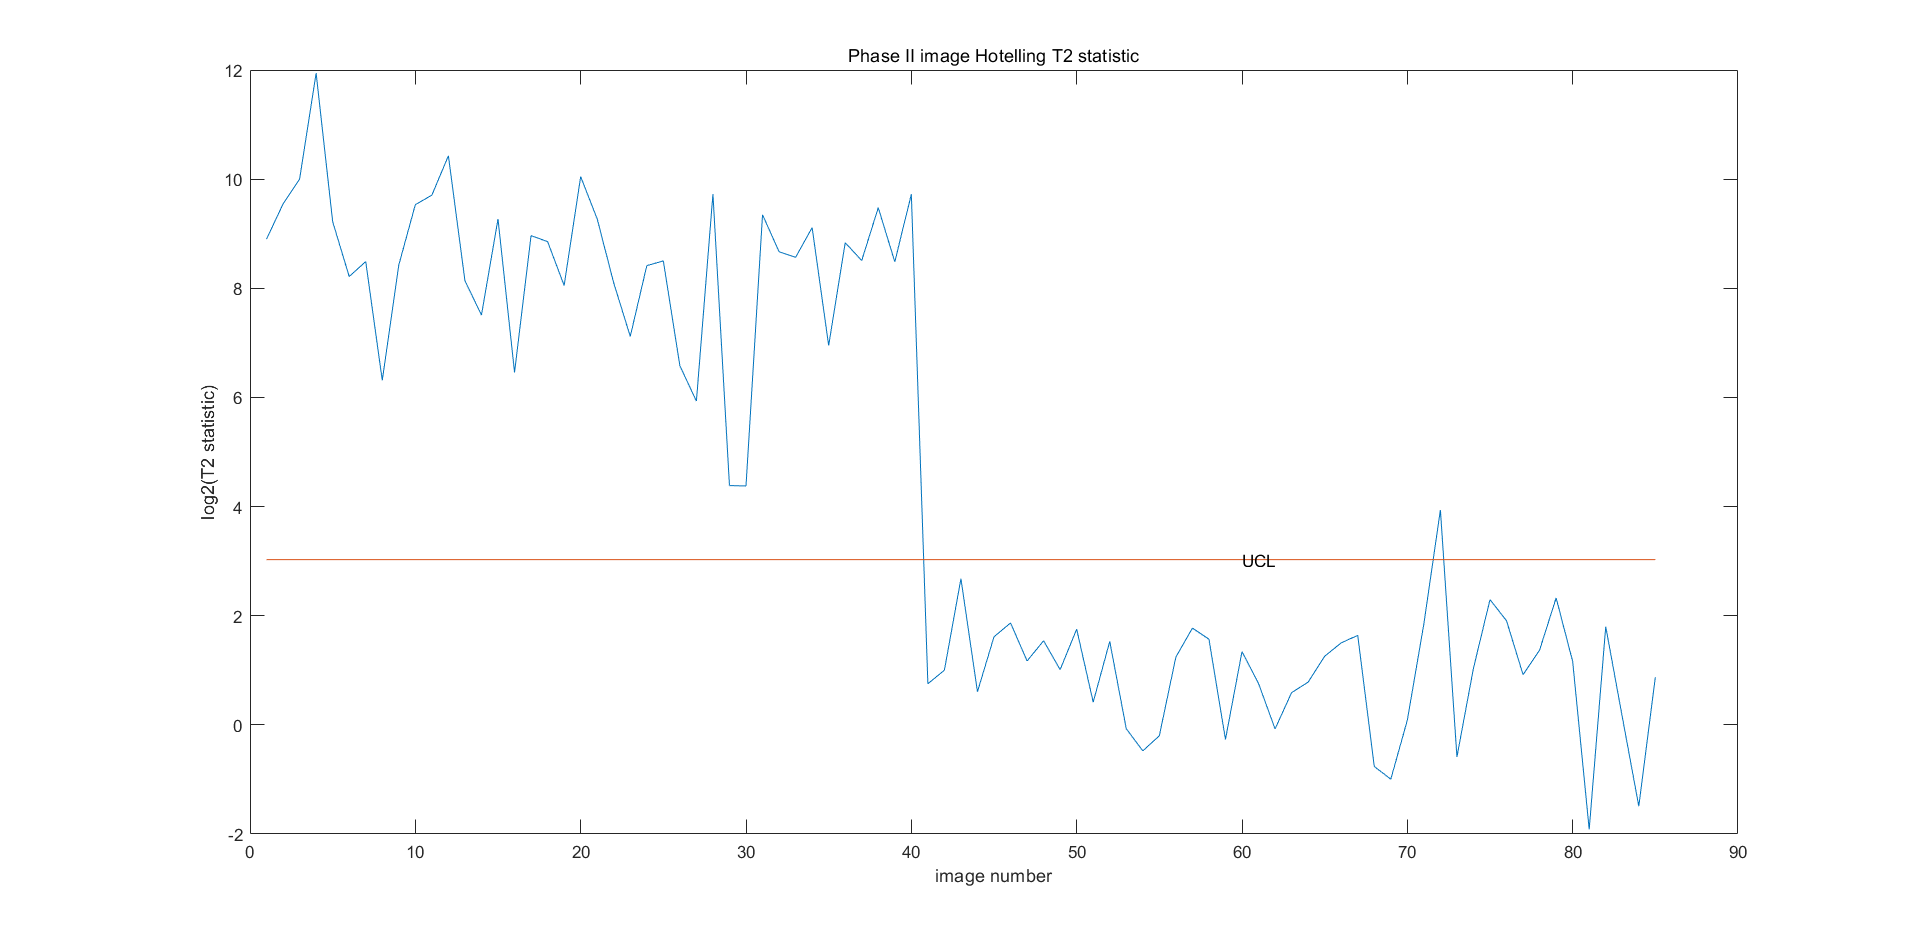
\includegraphics[width=\textwidth]{images/phaseII_t2.png}
         \caption{The Phase II wavelet decomposition based Hotelling $T^{2}$ control chart, where the first 40 images are sample with defects, other 45 are qualified samples. The orange line indicate the UCL and there are 1 false detection sample in the control chart.}
        \label{fig:T_result_d1}
    \end{subfigure}
\end{figure}



\newpage
\subsection{Application of two methods on different colour images}
This study aims to verify if the above mentioned two methods are suitable to detect defects without considering the image colour. To change the colour, we first convert an RGB image into an HSV (hue, saturation, and value) image, an $M\times N \times3$ numeric array with values in the range [0, 1]. The three dimensions of HSV (Figure~\ref{fig:hsv}) defines the hue, saturation, and brightness value for each pixel, respectively. The dimension hue describes value from 0 to 1 corresponding to the colour's position on a colour wheel. As hue increases from 0 to 1, the colour transitions from red to orange, yellow, green, cyan, blue, magenta, and finally back to red. As for saturation, it represents the amount of hue or departure from neutral. 0 indicates a neutral shade, whereas 1 indicates maximum saturation. And value works in conjunction with saturation and describes the brightness or intensity of the color, from 0 to 100 percent, where 0 is completely black, and 100 is the brightest and reveals the most color. We modify the value of the $V$ frame to change the colour of the image from blue to red, as shown in Figure~\ref{fig:color_change}.


\begin{figure}[h]
\centering
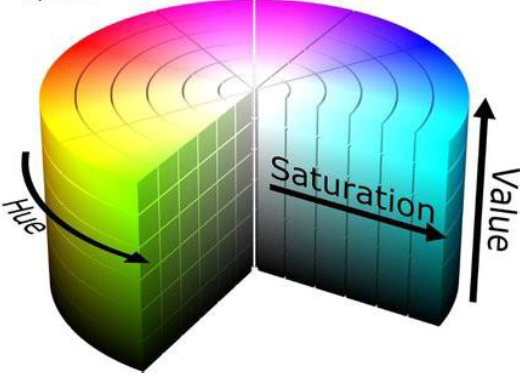
\includegraphics[width=0.75\textwidth]{images/hsv.PNG}
\caption{An Illustration of HSV dimention of an image.}
\label{fig:hsv}
\end{figure}

\begin{figure}[h]
\centering
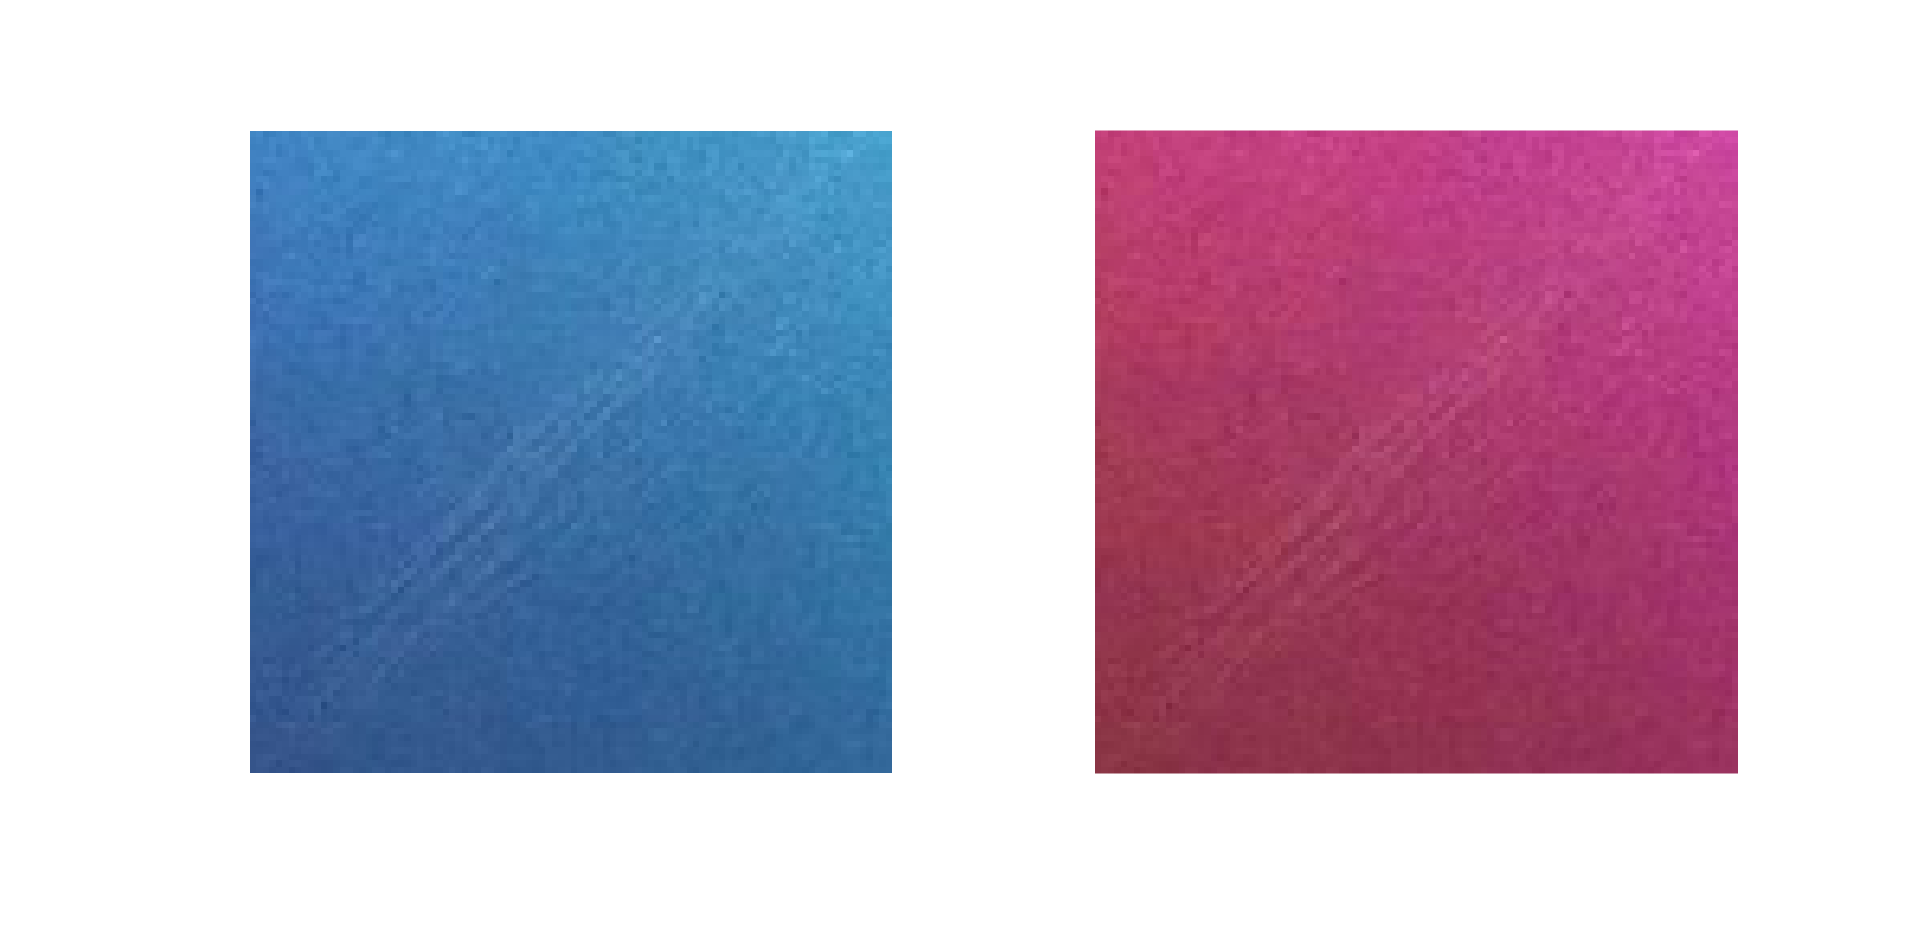
\includegraphics[width=0.75\textwidth]{images/color_change.png}
\caption{An example of defect image in different color. The left is the original image, the right one is the color changed image after HSV modification.}
\label{fig:color_change}
\end{figure}

To test the performance of two methods on different colour images, we first modify the brightness value of all samples and then repeat Phase I and Phase II procedure on all colour changed images as we have done in section~\ref{sec:5.3}. The control charts of Phase I are shown in Figure~\ref{fig:phasI_methodI_color} and ~\ref{fig:phasI_methodII_color}.

\begin{figure}
    \centering
    \begin{subfigure}{\textwidth}
         \centering
         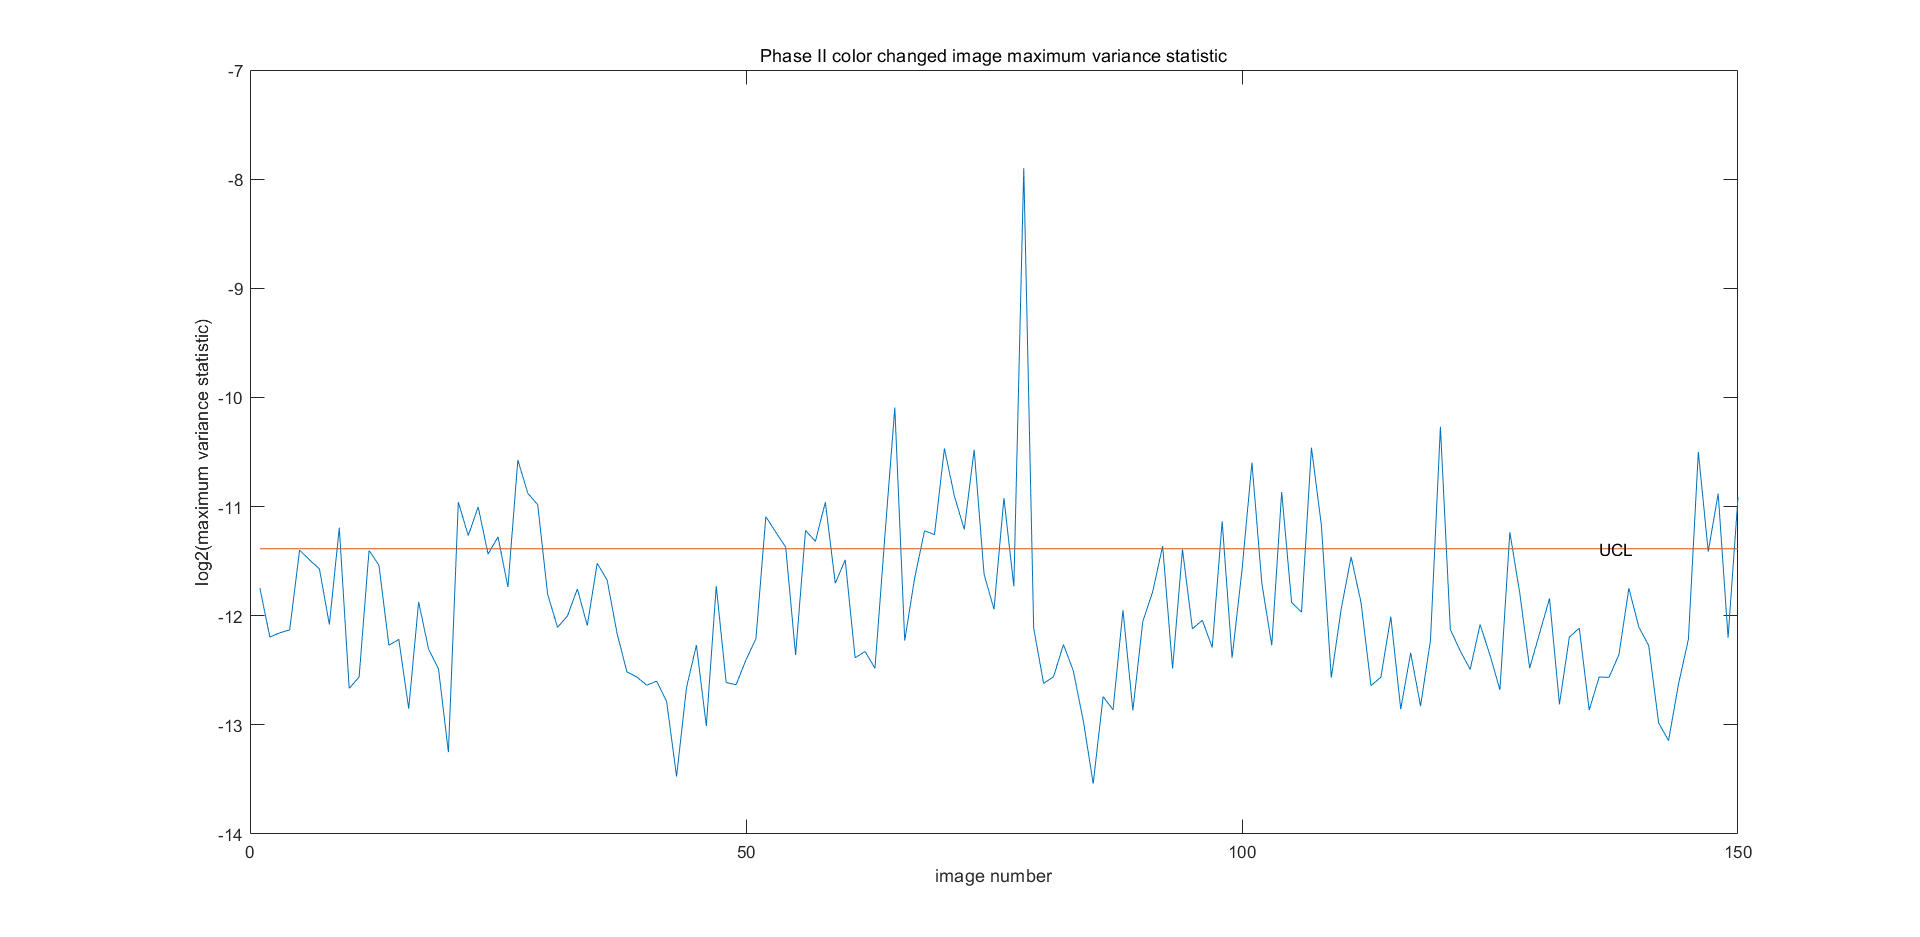
\includegraphics[width=\textwidth]{images/phaseI_color_max.png}
         \caption{The Phase I maximum variance based $\bar{X}$ control chart of red images, where all the samples are qualified and there are 35 false alarms in the control chart. The orange line is the UCL of $\bar{X}$ control chart}
        \label{fig:phasI_methodI_color}
    \end{subfigure}
     
    \begin{subfigure}{\textwidth}
         \centering
         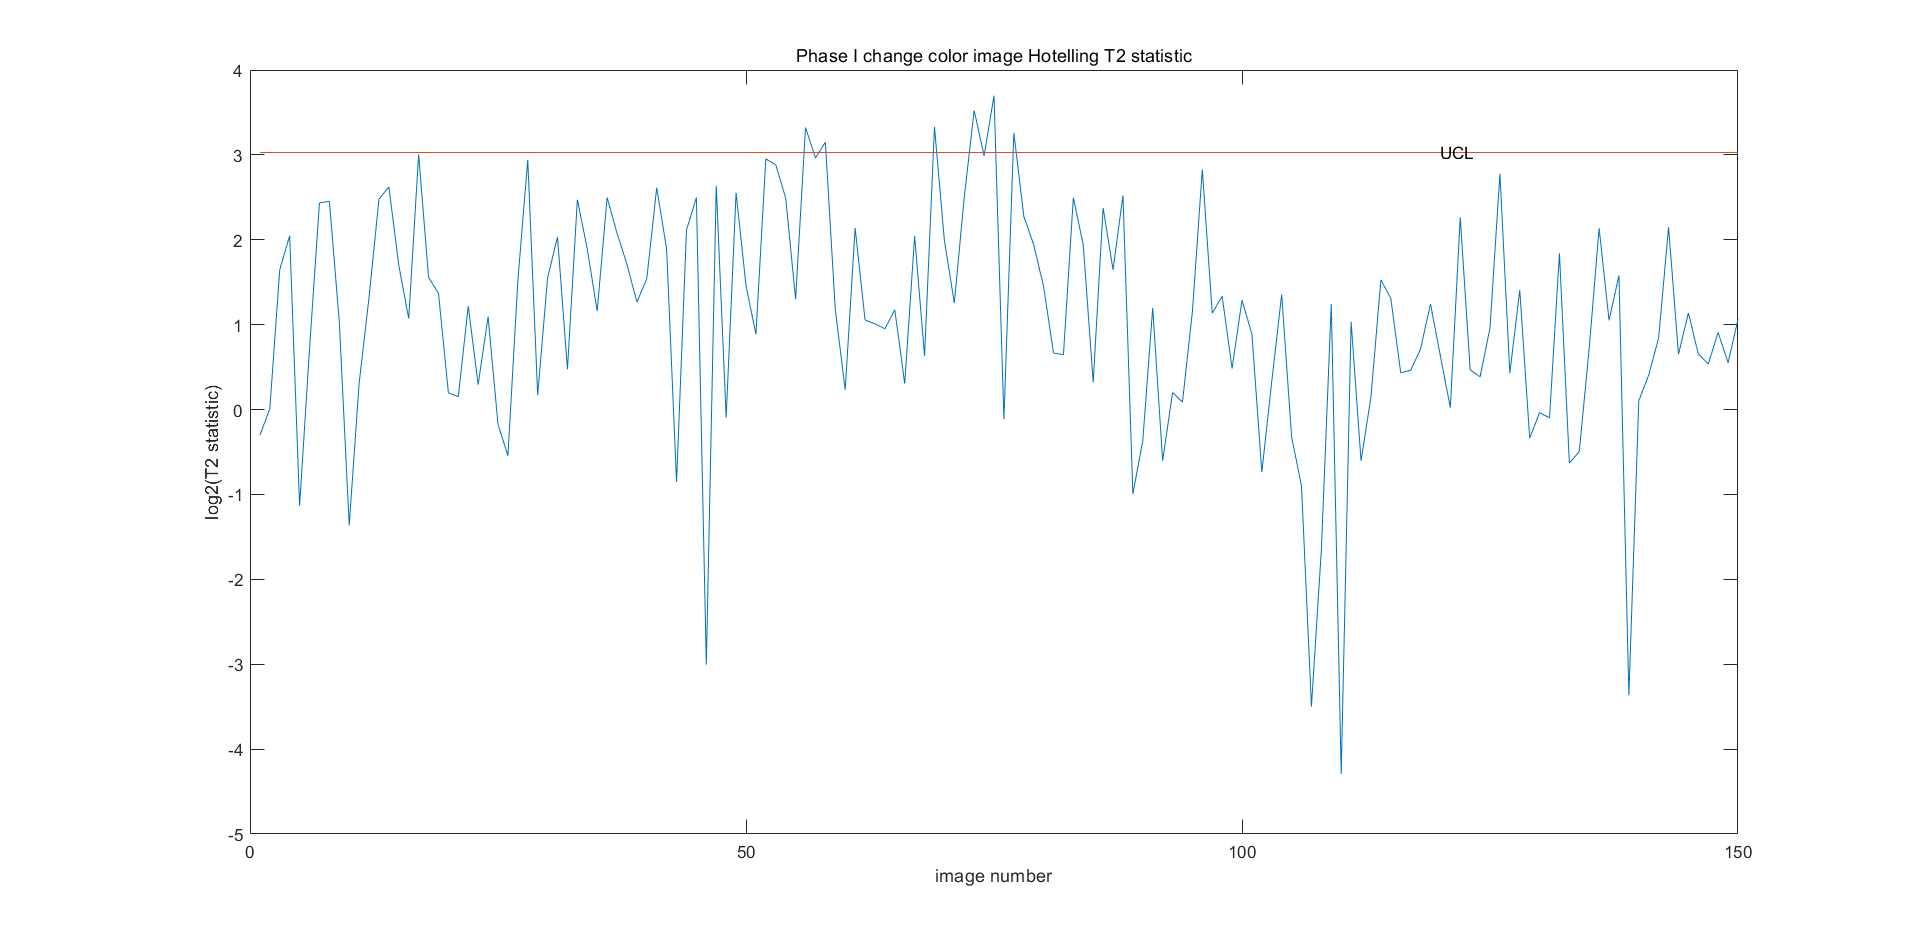
\includegraphics[width=\textwidth]{images/phaseI_color_t2.png}
         \caption{The Phase I wavelet decomposition based Hotelling $T^{2}$ control chart of red images, where all the samples are qualified and there are 6 false alarms in the control chart. The orange line is the UCL of Hotelling $T^{2}$ control chart}
        \label{fig:phasI_methodII_color}
    \end{subfigure}
\end{figure}

The mean value ($\overline{m}$) of maximum variance of changed colour image in Phase I is 3.123e-04, the standard deviation ($\sigma_{s}$) is 1.09e-04, thus the UCL and LCL is 3.735e-04 and 2.51e-04 respectively. By method II in Phase I the sample mean vector of Haar wavelet decomposition characteristic is
\begin{equation}
\centering
\overline{\mathbf{x}} = 
\begin{bmatrix}
0.229&	0.414&	0.085
\end{bmatrix}, 
\end{equation}


and the sample covariance matrix is
\begin{equation}
\centering
\mathbf{S} = 
\begin{bmatrix}
0.011	&  0.023	&  -0.00019\\
0.02303	&  0.0868 &	-0.00164\\
-0.00019 &	-0.00164 &	0.000639
\end{bmatrix},
\end{equation}

the UCL of colour changed image by method II is the same as that by original data, namely 8.157. The $ARL$ of method I and method II according to Equation (\ref{equ:arl}) is 4.286 and 25, respectively. 

The control charts of Phase II data of two methods are shown in Figure~\ref{fig:max_result_15errors} and \ref{fig:T_result_d1}. There are 4 and 2 false detections in method I and method II respectively, the corresponding false detection rate of method I is 4.7\%, for method II 2.35\%.



\begin{figure}
    \centering
    \begin{subfigure}{\textwidth}
         \centering
         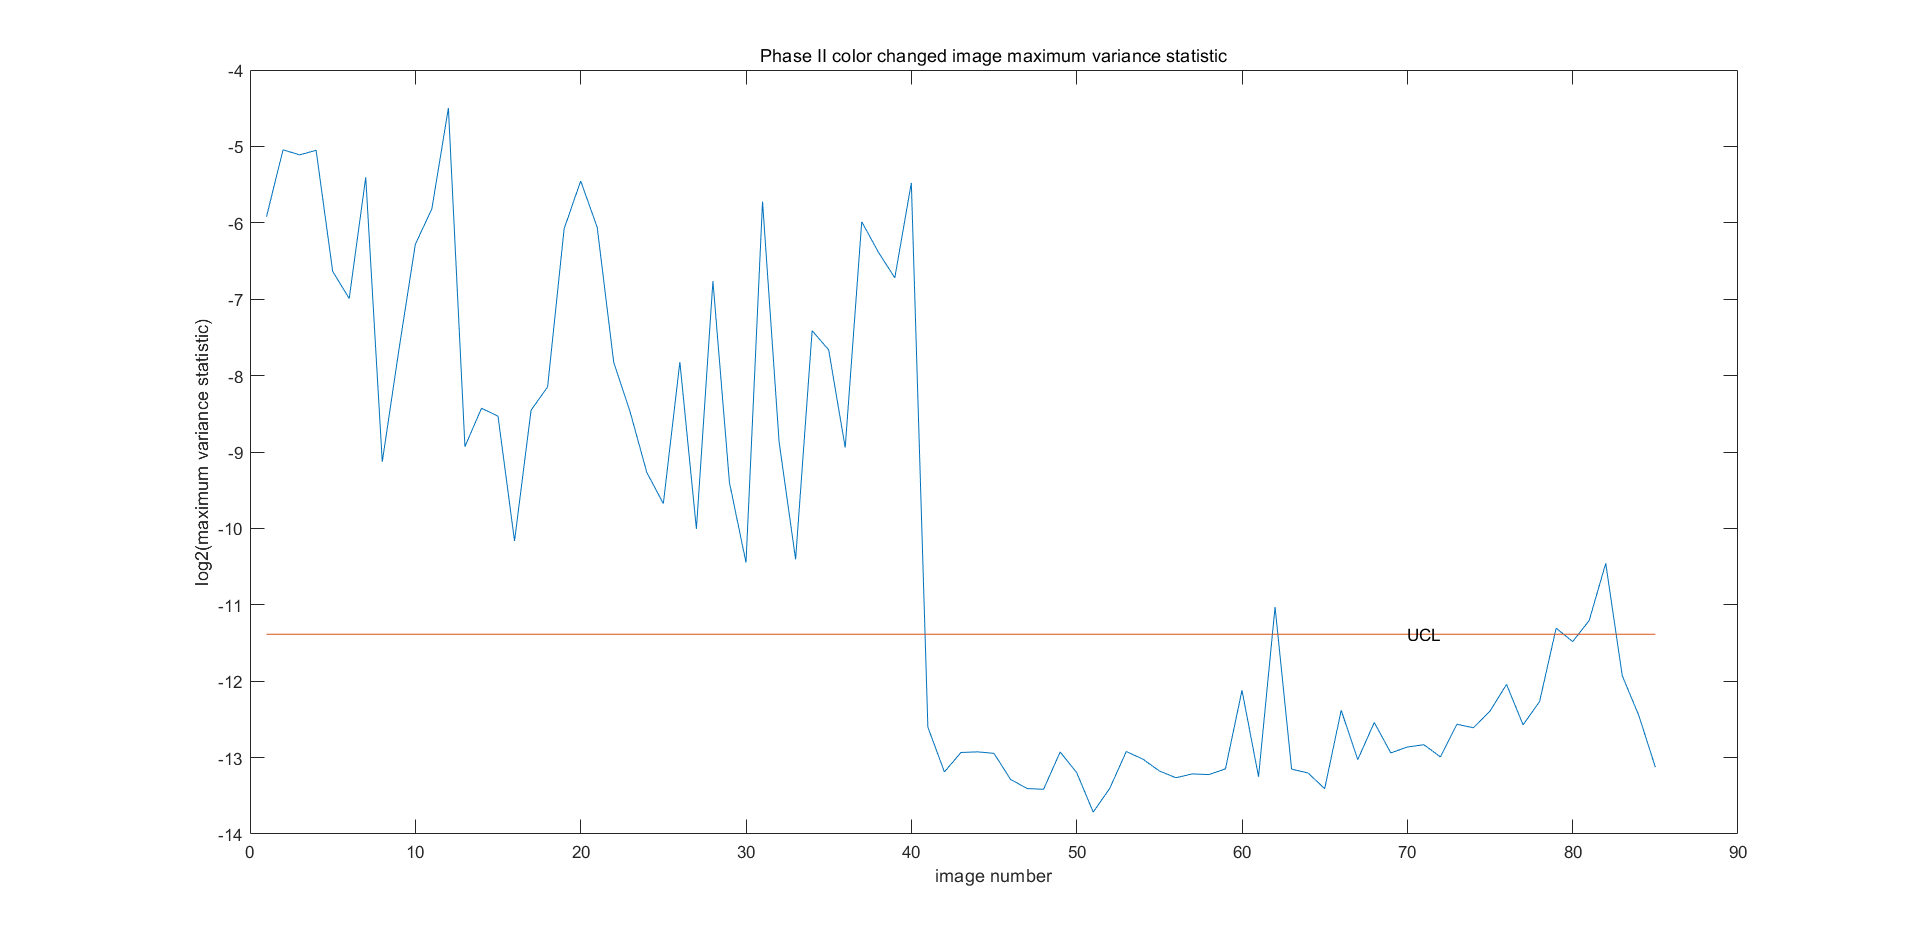
\includegraphics[width=\textwidth]{images/phaseII_color_max.png}
         \caption{The maximum variance based $\bar{X}$ control chart of red images in Phase II, where the first 40 images are sample with defects, other 45 are qualified samples. The orange line indicate the UCL and there are 4 false detection samples in the control chart.}
        \label{fig:max_result_15errors}
    \end{subfigure}
     
    \begin{subfigure}{\textwidth}
         \centering
         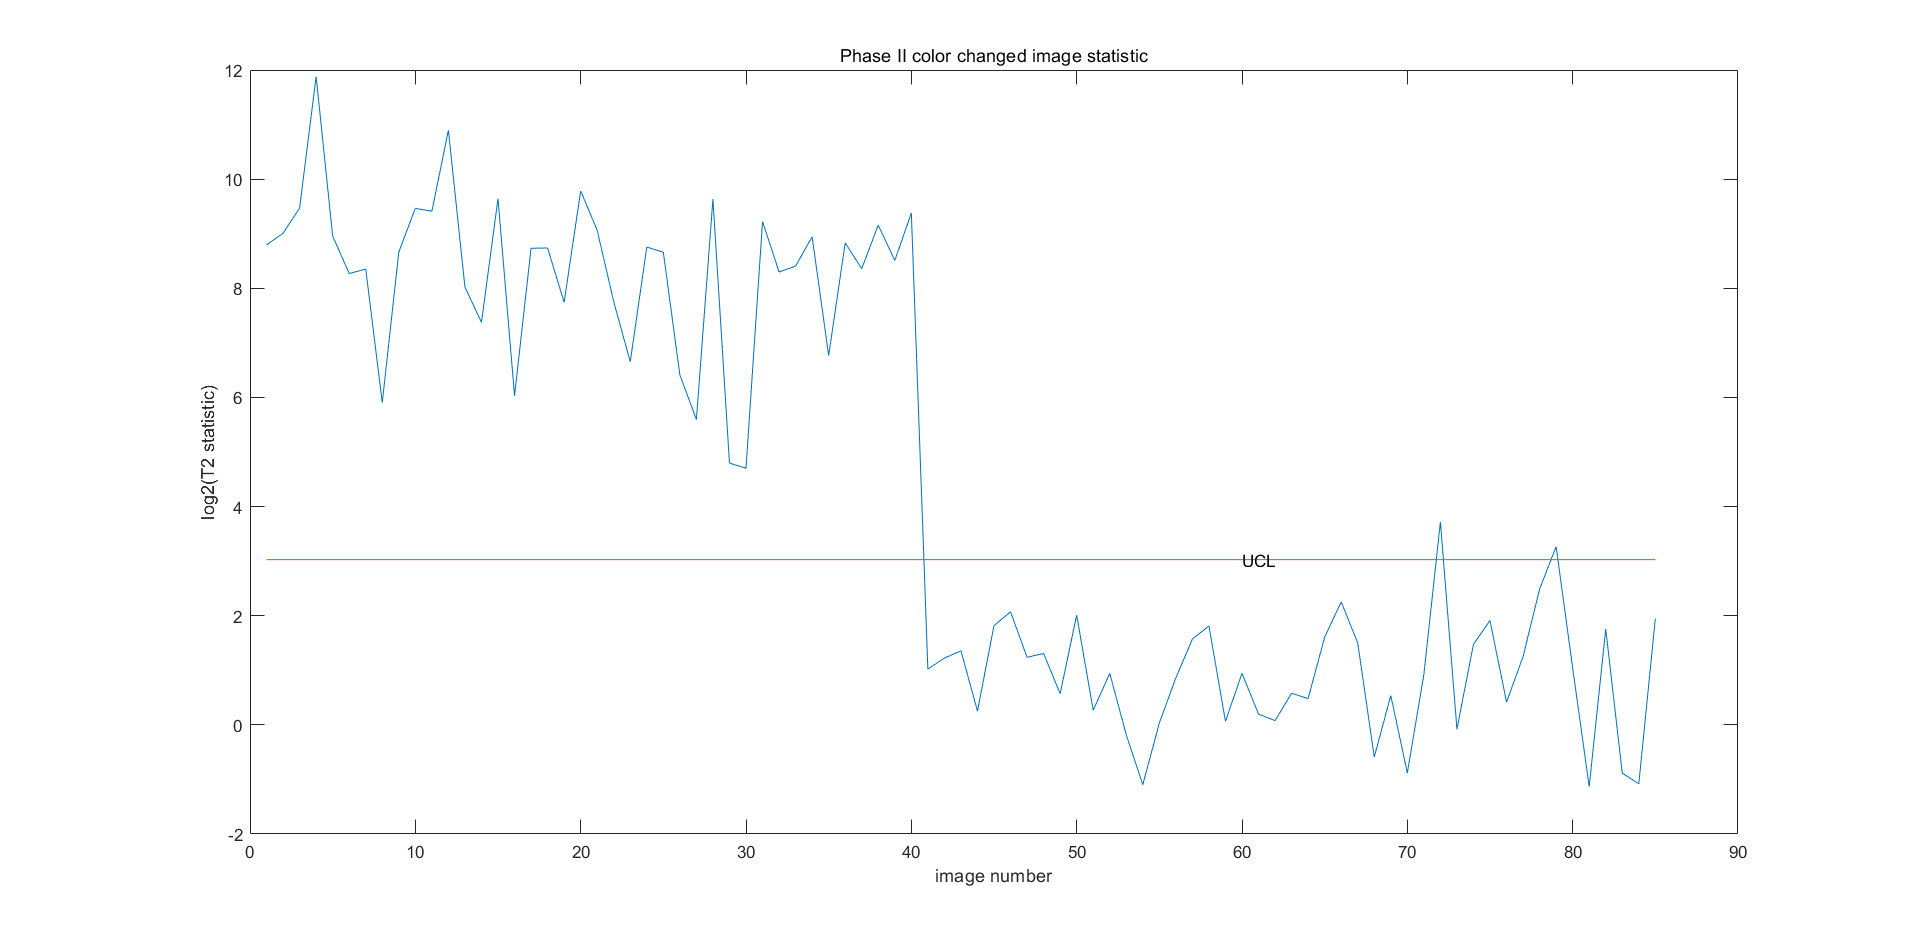
\includegraphics[width=\textwidth]{images/phaseII_color_t2.png}
         \caption{The wavelet decomposition based Hotelling $T^{2}$ control chart of red images in Phase II, where the first 40 images are sample with defects, other 45 are qualified samples. The orange line indicate the UCL and there are 2 false detection samples in the control chart.}
        \label{fig:T_result_d1}
    \end{subfigure}
\end{figure}

\begin{comment}
\begin{figure}[h]
\centering
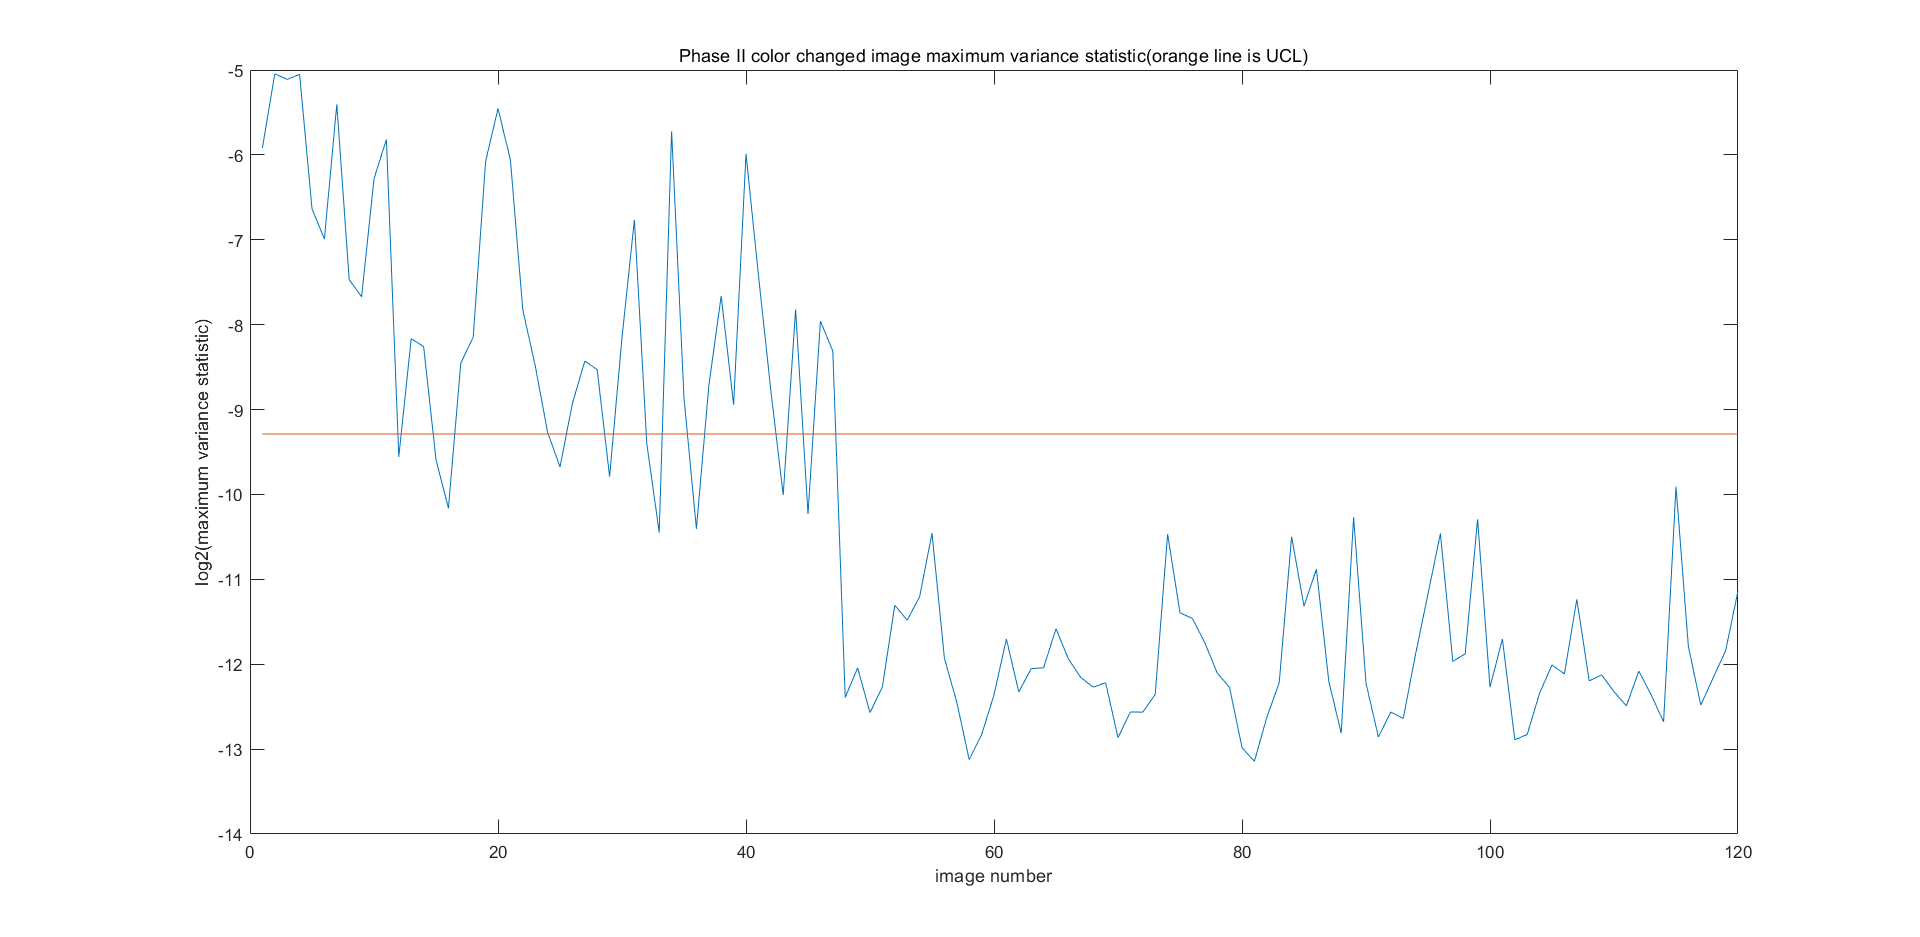
\includegraphics[width=1.0\textwidth]{images/log_max_color.png}
\caption{The maximum variance based $\bar{X}$ control chart of changed colour images, where the first 47 images are sample with defects, others are qualified samples. The orange line indicate the UCL and there are 10 false detection samples in the control chart.}
\label{fig:max_result_15errors}
\end{figure}

\begin{figure}[h]
\centering
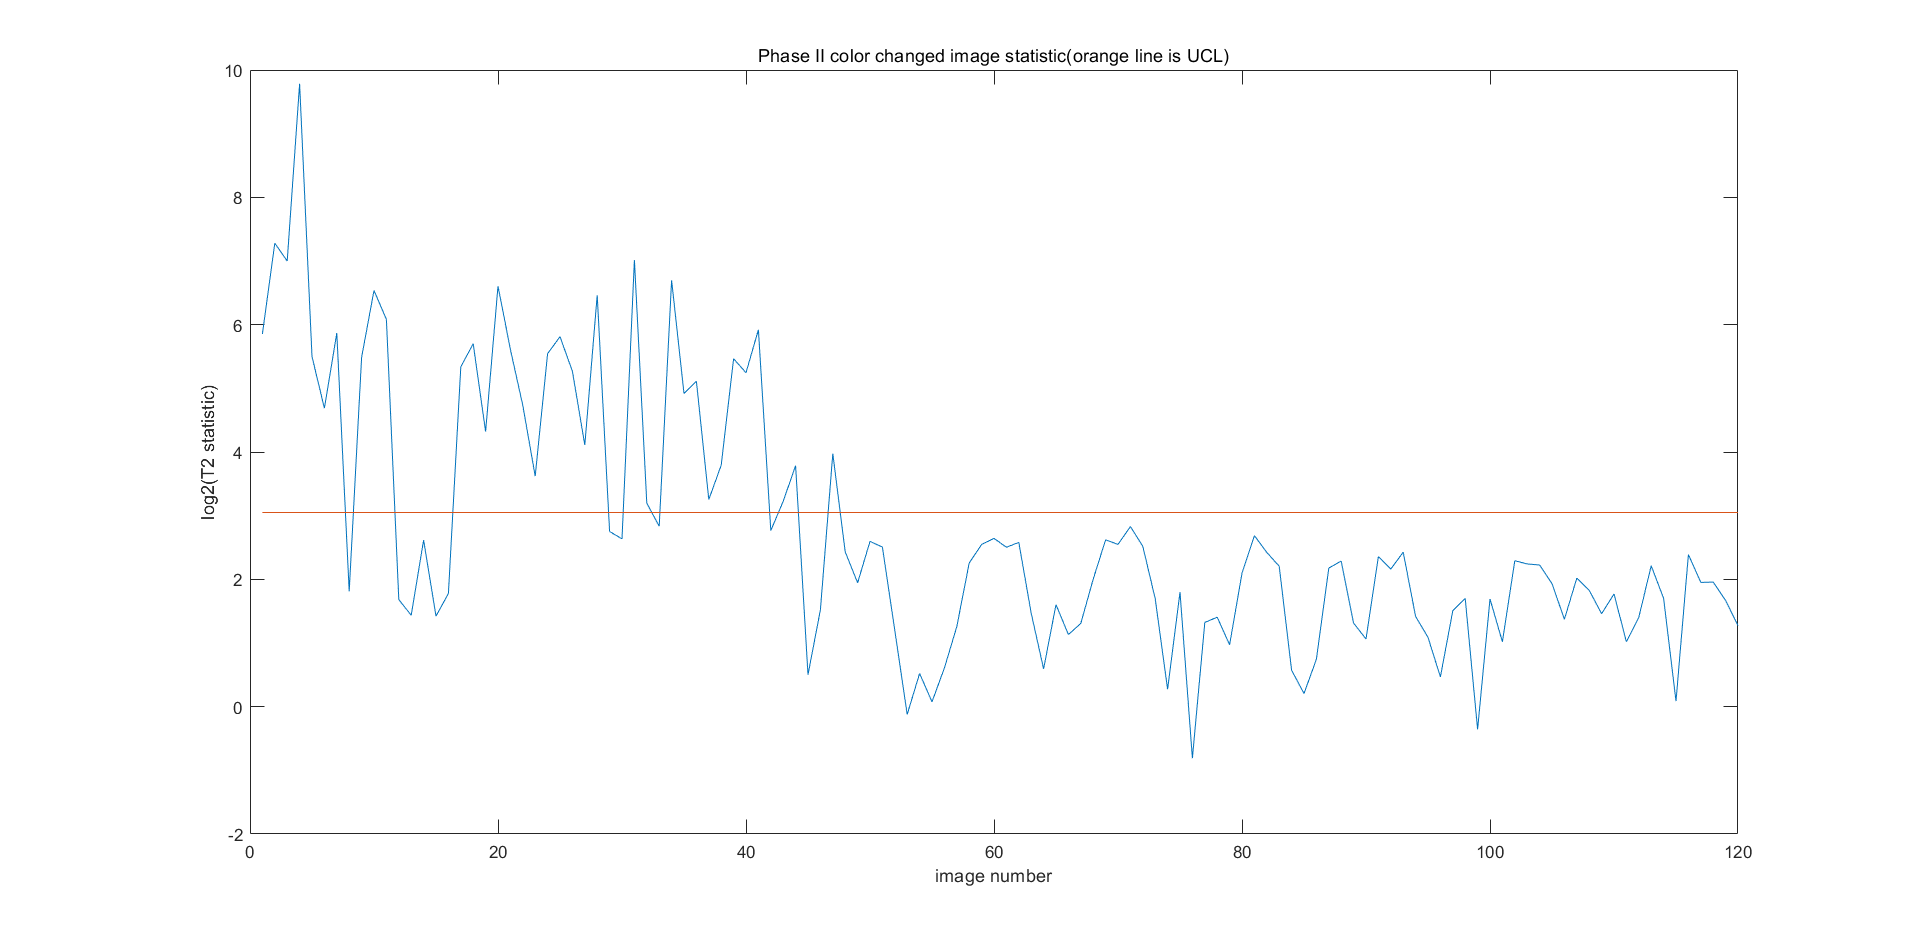
\includegraphics[width=1.0\textwidth]{images/log_t2_color.png}
\caption{The wavelet decomposition based Hotelling $T^{2}$ control chart of changed colour images, where the first 47 images are sample with defects, others are qualified samples. The orange line indicate the UCL and there are 12 false detection samples in the control chart.}
\label{fig:T_result_d1}
\end{figure}
\end{comment}

The experiment conducted above only verify that these methods work on other samples with different colour when we repeat Phase I and Phase II procedure. But assume we have a product, in our case the mobile phone cover, with different production lines with respect to different colour, can we use the derived in-control parameters from the samples of one colour e.g., blue, and apply these in-control parameters to the rest samples with different colour without repeat the Phase I procedure? Thus we conduct an other comparison experiment by using the parameter derived from Phase I of blue samples to monitor the red samples in Phase II. The result of the control charts is shown in Figure~\ref{fig:phase_II_max_use_blue_sample} and \ref{fig:phase_II_t2_use_blue_sample}. From the control chart we can see that method I fail to detect all the defect samples and method II fail to detect all standard samples, which indicate that the proposed framework is not suitable in mix colour defect detection.


\begin{figure}
    \centering
    \begin{subfigure}{\textwidth}
         \centering
         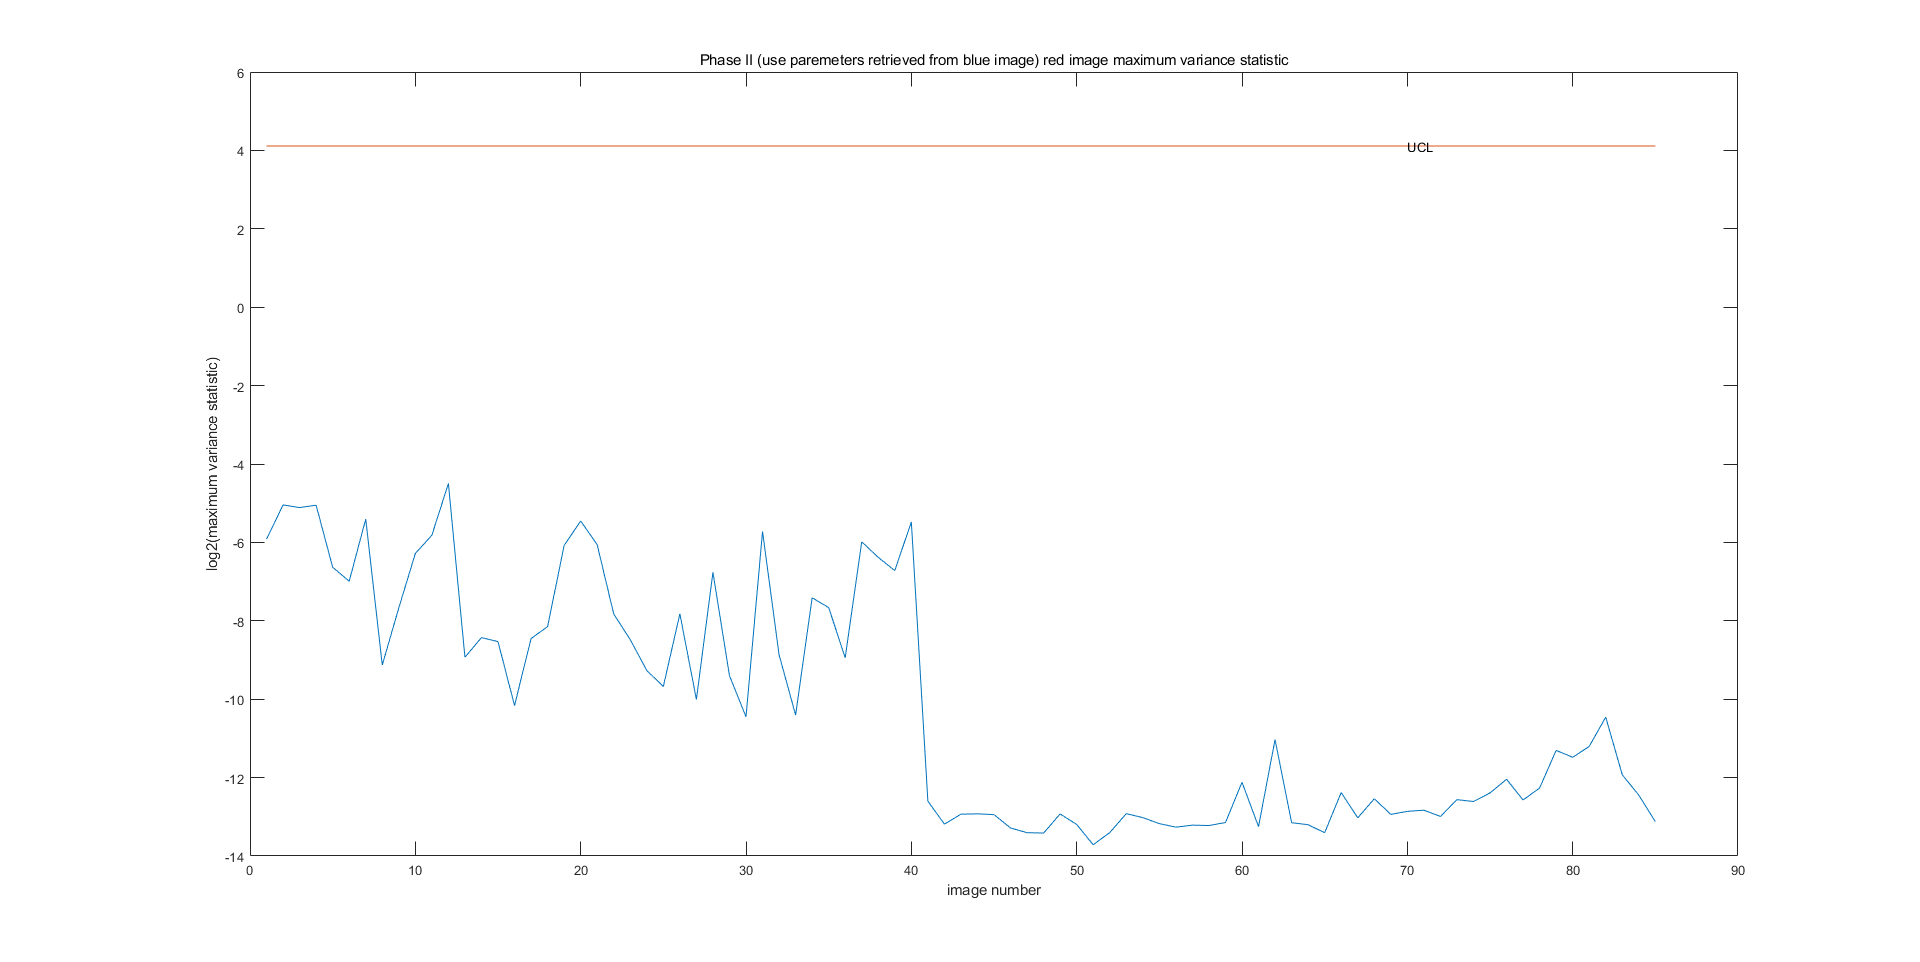
\includegraphics[width=\textwidth]{images/phase_II_max_use_blue_sample.png}
         \caption{The maximum variance based $\bar{X}$ control chart of red images in Phase II by using the parameter derived from Phase I of blue samples, where the first 40 images are sample with defects, other 45 are qualified samples. The orange line indicate the UCL and there are 40 false detection samples in the control chart.}
        \label{fig:phase_II_max_use_blue_sample}
    \end{subfigure}
     
    \begin{subfigure}{\textwidth}
         \centering
         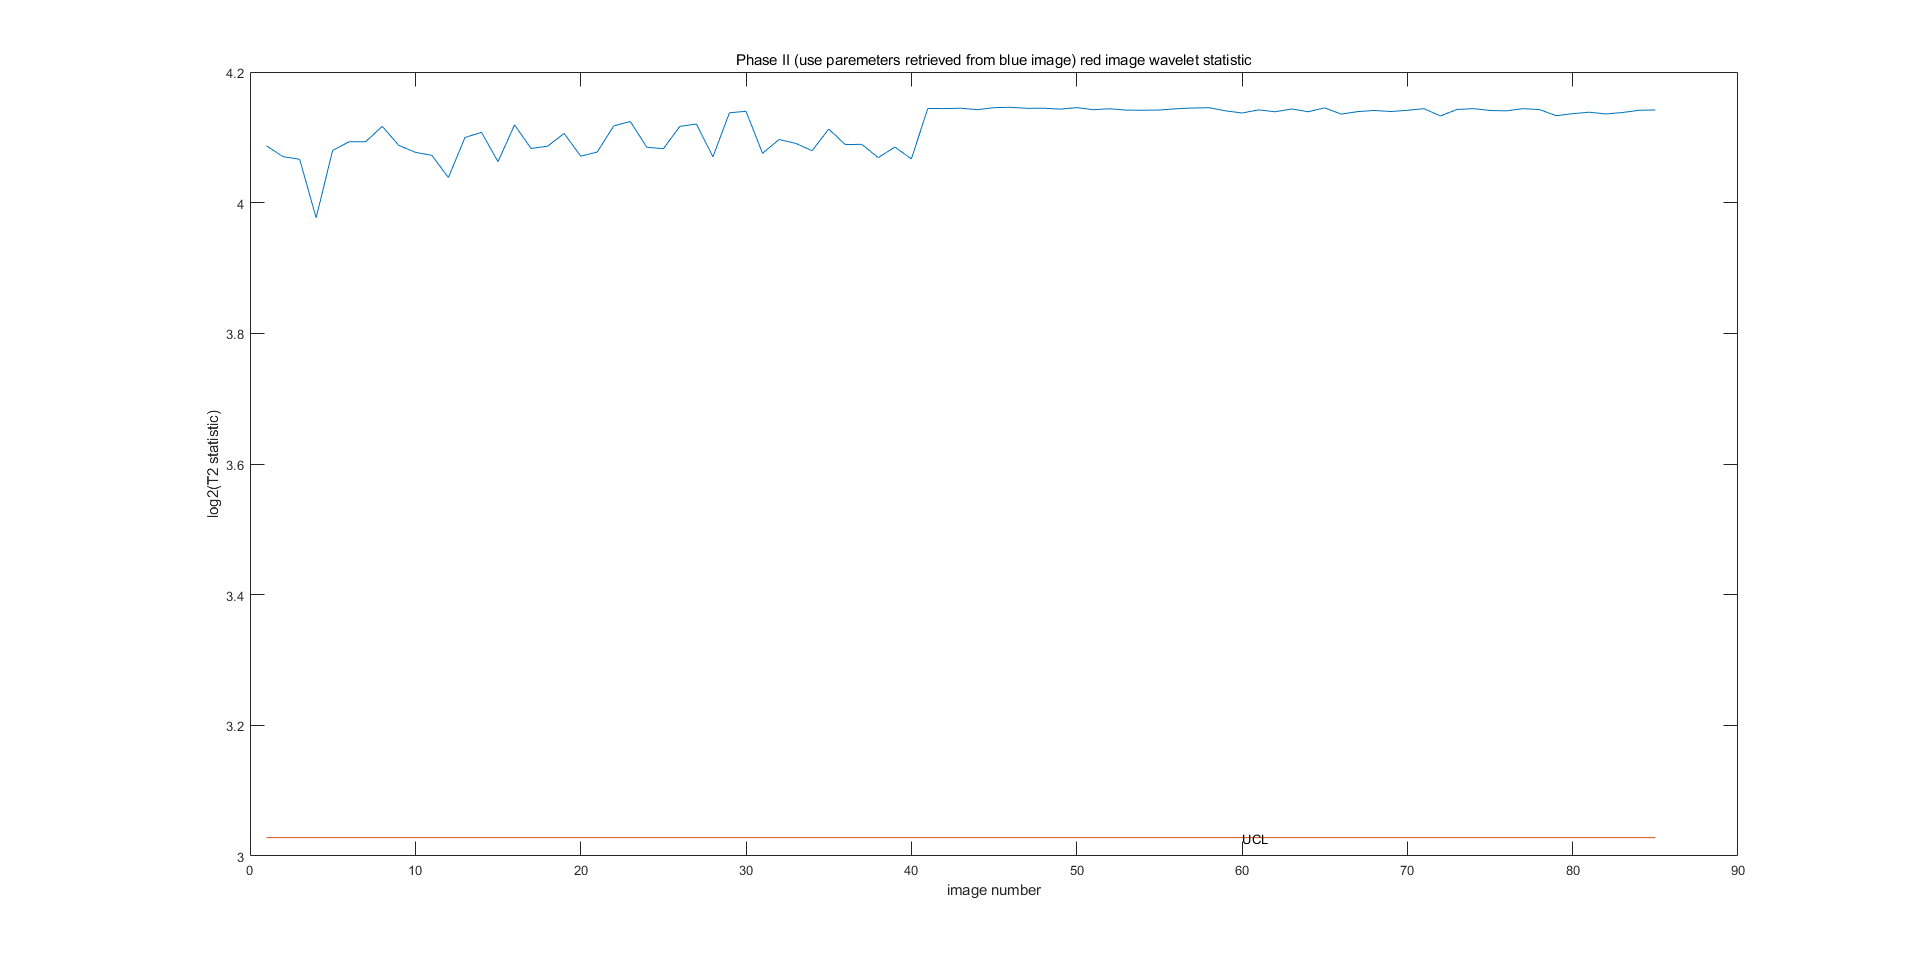
\includegraphics[width=\textwidth]{images/phase_II_t2_use_blue_sample.png}
         \caption{The wavelet decomposition based Hotelling $T^{2}$ control chart of red images in Phase II by using the parameter derived from Phase I of blue samples, where the first 40 images are sample with defects, other 45 are qualified samples. The orange line indicate the UCL and there are 45 false detection samples in the control chart.}
        \label{fig:phase_II_t2_use_blue_sample}
    \end{subfigure}
\end{figure}



\newpage
\section{Conclusion}
In this section we will summarize the results of empirical study and draw the conclusion. The result of the empirical study is shown in Table~\ref{tab:result_summary}

\begin{table}[htp]
\centering
\setlength{\tabcolsep}{0pt}
\begin{tabular*}{\textwidth}{
  @{\extracolsep{\fill}}
  l
  S[table-format=1.3e-2]
  S[table-format=6.0]
  S[table-format=1.4e-1]
  S[table-format=1.1]
  S[table-format=1.4e-1]
  @{}
}
\toprule
 &
Phase I $ARL$ &
Phase II $ASS$ &
Phase II $FDR$ \\
\midrule
method I & 3.13 & 27.42 & 5.8\%  \\
method II & 30 & 67.12 & 1.1\%  \\
method I (different colour) & 4.28 & 27.9 & 4.7\%  \\
method II (different colour) & 25 & 62.7 & 2.3\%  \\
method I (mix colour) & \slash & \slash & 47.05\%  \\
method II (mix colour) & \slash & \slash & 52.94\%  \\
\bottomrule
\end{tabular*}
\caption{The summary result of control charts in different methods. The table shows the different performance variable of two methods.}
\label{tab:result_summary}
\end{table}

As is shown in the table, the $ARL$ of method II is ten times that of method I, while the $FDR$ of method II is five times smaller than that of method I, which lead to the conclusion that method II achieve better performance in defects detection. Regarding the $ASS$, method II is almost twice as much as method I, which indicates that method II is more sensitive to defects than method I. By comparing the $ARL$, $FDR$, and $ASS$ of colour images and standard images, we can see that there is a slight difference between two forms of image, from which we can conclude that the performance of control chart by faults detection is independent from colour of samples when we apply each samples set Phase I and Phase II. However, when we apply the from one sample set derived in-control parameters to another sample set, both methods fail to detect faults ($FDR$ 47.05\% and 52.94\% respectively). The reason may be the way to generate the red sample in our study, namely, we modify the Hue value of the original image to change the colour of the images, which leads to pixel value change. Thus the in-control parameters and $UCL$ retrieved from other samples fail to work on Phase II.





























